\subsection{Object Document Mapper (ODM) Diagram}
\label{subsec:odm_subsec}
Since the database that will be developed for the system will be 
a non-relational, hence an Object Document Mapper (ODM) 
diagram is shown in this section rather than an Entity Relationship Diagram (ERD).
\vspace{0.5cm}
\\The ODM diagram is shown in Figure \ref{fig:odm}:
\begin{figure}[ht]
    \centering
    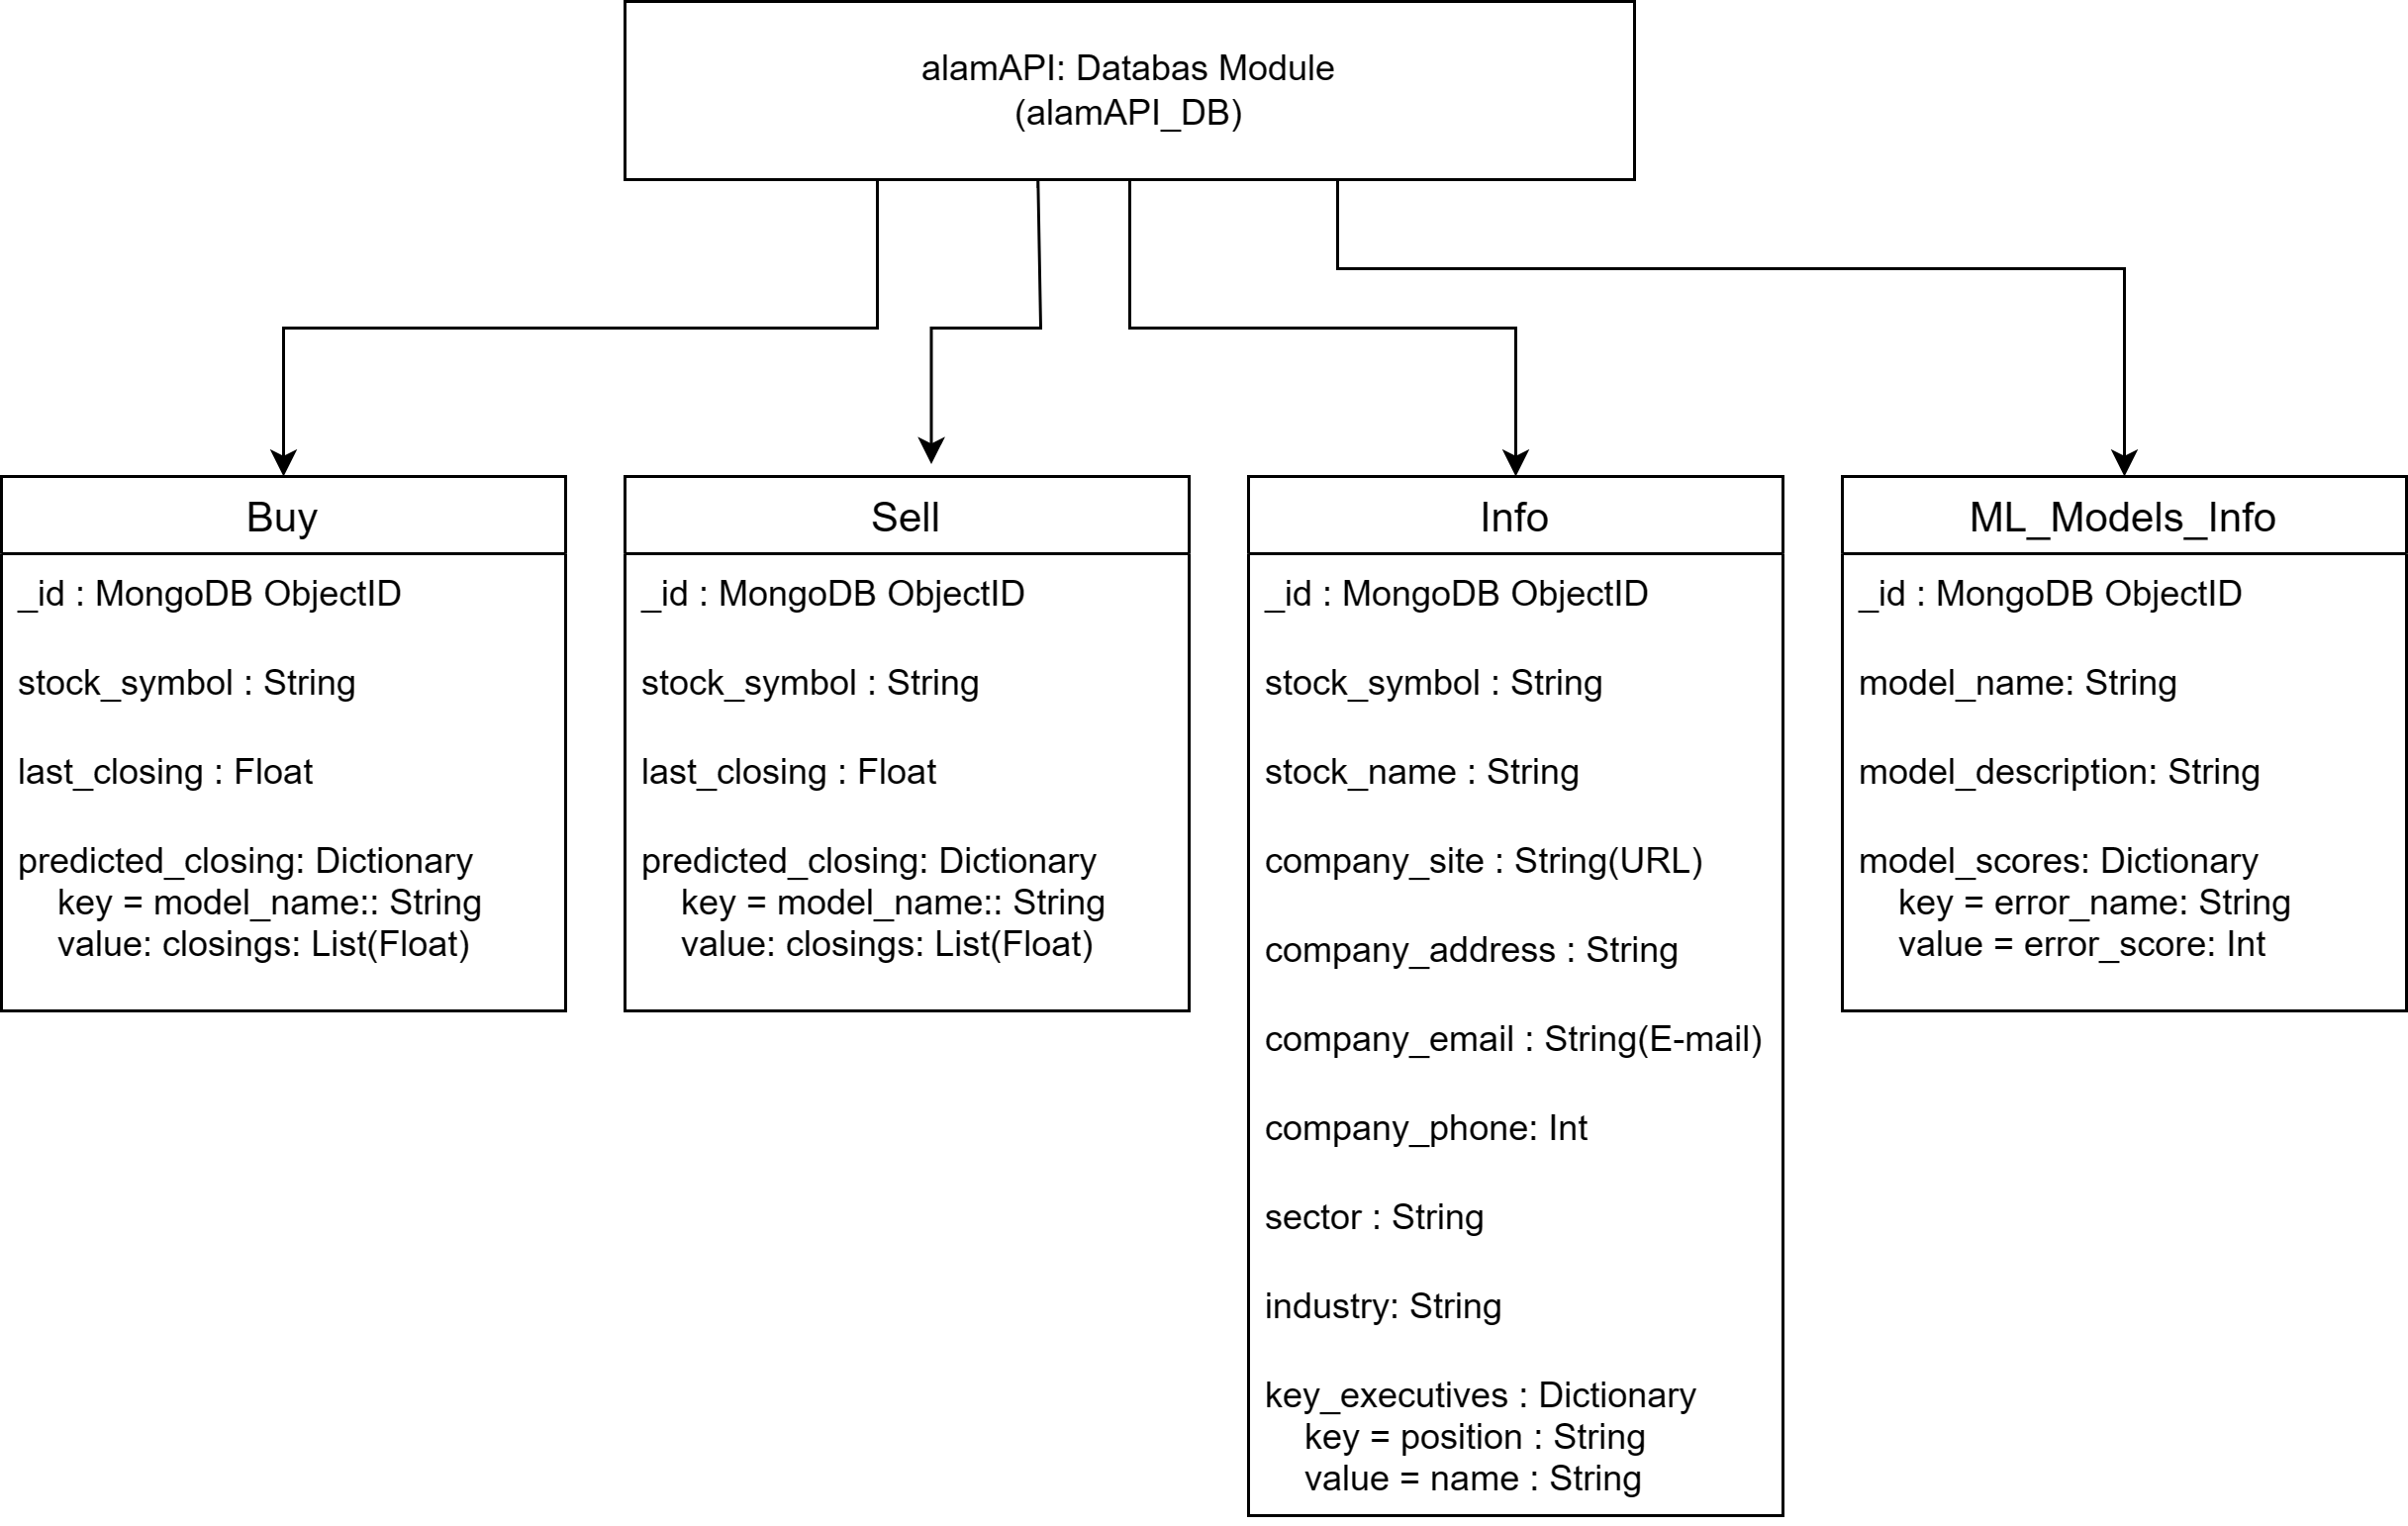
\includegraphics[width=1\textwidth]{./assets/ODM.png}
    \caption{Object-Data-Model for the alamAPI}
    \label{fig:odm}
\end{figure}
\FloatBarrier
As shown from the Figure \ref{fig:odm}, the SMPTFSys\_DB will be the collection
name of the non-relational database of the system. Wherein it 
will be composed of three documents with the list items following this convention: 
“item name”: “item type”. 
Note that each document are their own separate entities, 
hence the database is called non-relational, as the documents are not in 
any way related to each other.
\vspace{0.5cm}
\\The three documents are as follows:
\begin{itemize}
    \item[(a)] Buy – this document will contain all the stocks that 
    the machine learning model predicted and classified as a stock to buy. 
    The diagram shown in Figure \ref{fig:odm} also tells the path in which this 
    document can be accessed, that is: $$ MongoDB Instance \rightarrow SMPTFSys_DB 
    \rightarrow Buy$$ Wherein, information regarding the stocks can be accessed using 
    the stock\_symbol, since the \_id is a private id.
    \item[[b)] Sell – this document will contain all the stock that the 
    machine learning model predicted and classifies as a stock to sell. 
    The diagram shown in \ref{fig:odm} also tells the path in which this 
    document can be accessed, that is: $$ MongoDB Instance \rightarrow 
    SMPTFSys_DB \rightarrow Sell$$
     Wherein, information regarding the stocks can be accessed using the 
     stock\_symbol, since the \_id is a private id.
    \item[(c)] Info – this document will contain the general and relevant 
    information about a stock, or the general company information. 
    The diagram shown in \ref{fig:odm} also tells the path in which this 
    document can be accessed, that is: 
    $$ MongoDB Instance \rightarrow SMPTFSys_DB \rightarrow Info $$ 
    Wherein, information regarding the stocks can be accessed using the 
    stock\_symbol, since the \_id is a private id.
\end{itemize}